\let\negmedspace\undefined
\let\negthickspace\undefined
\documentclass[journal]{article}
\usepackage[a5paper, margin=10mm, onecolumn]{geometry}
\usepackage{lmodern} % Ensure lmodern is loaded for pdflatex

\setlength{\headheight}{1cm} % Set the height of the header box
\setlength{\headsep}{0mm}     % Set the distance between the header box and the top of the text

\usepackage{gvv-book}
\usepackage{gvv}
\usepackage{cite}
\usepackage{textcomp}
\usepackage{amsmath,amssymb,amsfonts,amsthm}
\usepackage{algorithmic}
\usepackage{graphicx}
\graphicspath{{./figs/}}
\usepackage{textcomp}
\usepackage{xcolor}
\usepackage{txfonts}
\usepackage{listings}
\usepackage{enumitem}
\usepackage{mathtools}
\usepackage{gensymb}
\usepackage{comment}
\usepackage[breaklinks=true]{hyperref}
\usepackage{tkz-euclide} 
\usepackage{listings}
\usepackage{gvv}                                        
\def\inputGnumericTable{}                                 
\usepackage[latin1]{inputenc}                                
\usepackage{color}                                            
\usepackage{array}                                            
\usepackage{longtable}                                       
\usepackage{calc}                                             
\usepackage{multirow}                                         
\usepackage{hhline}                                           
\usepackage{ifthen}                                           
\usepackage{lscape}
\usepackage{circuitikz}
\tikzstyle{block} = [rectangle, draw, fill=blue!20, 
text width=4em, text centered, rounded corners, minimum height=3em]
\tikzstyle{sum} = [draw, fill=blue!10, circle, minimum size=1cm, node distance=1.5cm]
\tikzstyle{input} = [coordinate]
\tikzstyle{output} = [coordinate]


\begin{document}
	
	\bibliographystyle{IEEEtran}
	\vspace{3cm}
	
\title{8.2.12}
\author{EE25BTECH11047 - RAVULA SHASHANK REDDY}
\maketitle
\hrulefill
\bigskip 

\renewcommand{\thetable}{\theenumi}
\setlength{\intextsep}{10pt}

\textbf{Question:} \\

Find the parameters of the conic
\begin{align*}
   36x^2+4y^2=144. 
\end{align*}

\textbf{Solution:}
\begin{align}
g(\vec{x}) &= \vec{x}^\top \vec{V} \vec{x} + 2\vec{u}^\top \vec{x} + f = 0 \\
\vec{V} &= \myvec{36 & 0 \\ 0 & 4}, \quad 
\vec{u}=\myvec{0\\0}, \quad 
f=-144\\
\lambda_1 &= 36, \quad \lambda_2 = 4 \\
\end{align}

Since $\lambda_1 > \lambda_2$, apply affine transformation
\begin{align}
\vec{P} &= \myvec{0 & 1 \\ 1 & 0}, \quad \vec{x} = \vec{P}\vec{y}
\end{align}

Hence,
\begin{align}
\lambda_1 &= 4, \quad \lambda_2 = 36 \\
\vec{e}_1 &= \vec{p}_2 = \myvec{0\\1}, \quad
\vec{e}_2 = \vec{p}_1 = \myvec{1\\0}\\
f_0 &= \vec{u}^\top \vec{V}^{-1}\vec{u} - f = 144\\
e &= \sqrt{1-\frac{\lambda_1}{\lambda_2}}
= \sqrt{1-\frac{4}{36}}
= \frac{2\sqrt{2}}{3}\\
\text{Major axis} &= 2\sqrt{\frac{f_0}{\lambda_1}}
= 12 \\
\text{Minor axis} &= 2\sqrt{\frac{f_0}{\lambda_2}}
= 4
\end{align}
Normal vector of directrix:
\begin{align}
\vec{n} &= \sqrt{\lambda_2}\,\vec{p}_2 
= \sqrt{36}\myvec{0\\1} 
= \myvec{0\\6}\\
\vec{p}_1 &= \myvec{1\\0}, \quad \vec{p}_2 = \myvec{0\\1}
\end{align}
\begin{align}
c &= \frac{e\,\vec{u}^\top\vec{n} \;\pm\; 
\sqrt{\,e^{2}\left(\vec{u}^\top\vec{n}\right)^{2} 
- \lambda_{2}\left(e^{2}-1\right)\left(\|\vec{u}\|^{2}-\lambda_{2}f\right)}}{\lambda_{2}e\left(e^{2}-1\right)} \\[6pt]
c &= \pm\frac{1}{e}\sqrt{\frac{\lambda_2 f_0}{\lambda_1}}
= \pm\frac{1}{e}\sqrt{\frac{36\cdot144}{4}}
= \pm 27\sqrt{2} \\[6pt]
\end{align}
Foci:
\begin{align}
\vec{F} &= \frac{c e^2 \vec{n} - \vec{u}}{\lambda_2} \\
&= \pm 4\sqrt{2}\vec{e}_2
\end{align}

Directrices:
\begin{align}
\vec{n}^\top \vec{x} &= c \\
\vec{n}^\top \vec{x} &= \pm 27\sqrt{2}\\
6\vec{e_2}^\top \vec{x} &= \pm 27\sqrt{2}\\
\vec{e_2}^\top \vec{x} &= \pm \frac{9\sqrt{2}}{2}
\end{align}


Latus rectum:
\begin{align}
l &= \frac{2\sqrt{|f_0 \lambda_1|}}{\lambda_2}
= \frac{4}{3}
\end{align}

\[
\begin{array}{|c|c|}
\hline
\text{Parameter} & \text{Value} \\
\hline
\vec{V},\;\vec{u},\;f & 
\myvec{36 & 0\\0 & 4}, \; \vec{0}, \; -144 \\
\hline
\lambda_1,\lambda_2 & 4,\;36 \\
\hline
f_0 & 144 \\
\hline
e & \tfrac{2\sqrt{2}}{3} \\
\hline
\text{Major axis length} & 12 \\
\hline
\text{Minor axis length} & 4 \\
\hline
\text{Foci} & \vec{F}=\pm 4\sqrt{2}\,\vec{e}_2 \\
\hline
\text{Directrices} & \vec{e}_2^\top \vec{x} = \pm \tfrac{9\sqrt{2}}{2} \\
\hline
\text{Latus rectum} & \tfrac{4}{3} \\
\hline
\end{array}
\]
\newpage
\begin{figure}
    \centering
    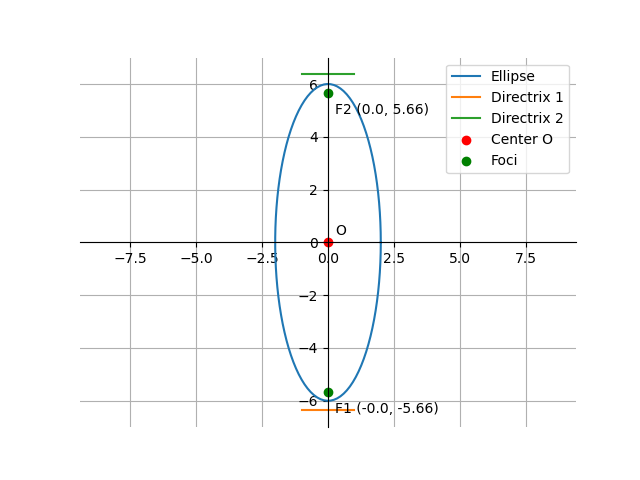
\includegraphics[width=1.0\linewidth]{figs/Figure_1.png}
    \caption{}
    \label{fig:placeholder}
\end{figure}
\end{document}

